\documentclass{article}
\usepackage{tikz}
\usepackage{smartdiagram}
\usepackage{metalogo, dtk-logos}
\begin{document}
	
\section{Primeiros Passos em Tikz}
	\begin{tikzpicture}[auto, node distance = 3cm,% 
	every node/.style={circle, draw, font = \sffamily\Large\bfseries}]
	\node (1) {1};
	\node (2) [below left of = 1] {2};
	\node (3) [below right of = 2] {3};
	\node (4) [below right of = 1] {4};
	\end{tikzpicture}\\
	

	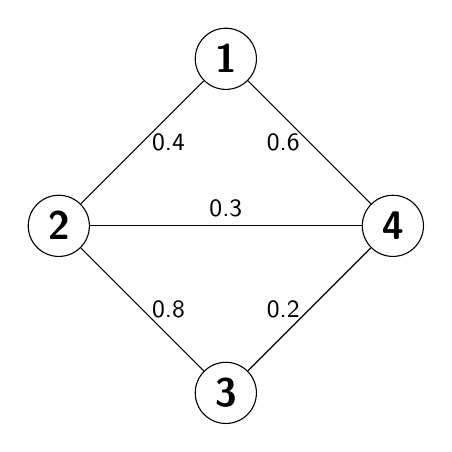
\begin{tikzpicture}[auto, node distance = 3cm,% 
	every node/.style={circle, draw, font = \sffamily\Large\bfseries}]
	\node (1) {1};
	\node (2) [below left of = 1] {2};
	\node (3) [below right of = 2] {3};
	\node (4) [below right of = 1] {4};

	\path[every node/.style={font=\sffamily\small}]
	(1) edge node [left]	{0.6} (4)
	(2) edge node [right]	{0.4} (1)
		edge node 			{0.3} (4)
	(3) edge node [right]	{0.8} (2)
	(4) edge node [left]	{0.2} (3);
	\end{tikzpicture}
	
\section{Ambiente Matrix}

\section{Diagramas}
\smartdiagram[flow diagram:horizontal]{Edit, \LaTeX, Bib\TeX/ biber, make\-index, \LaTeX}\\

\smartdiagram[circular diagram:clockwise]{
	Edit,
	pdf\LaTeX,
	Bib\TeX/ biber,
	make\-index,
	pdf\LaTeX}\\

\smartdiagram[bubble diagram]{\TeX\ engines,
\TeX\ (dvi),
pdf\TeX,
\XeTeX,
\LuaTeX,
Con\TeX t}\\

\smartdiagram[constellation diagram]{
\TeX\ software,
Editor,
Compiler,
Converter,
PDF Reader}\\


\smartdiagram[descriptive diagram]{
{Style,{Define shapes, colors, shading, and line styles for nodes and arrows}},
{Position,{Place nodes using a matrix, relative or absolute positioning}},
{Relation, Insert edges or arrows between selected nodes},
{Label, Add labels on edges or arrows}}\\

\smartdiagram[priority descriptive diagram]{
Develop a document structure,
Chosse a document class,
Select suitable packages,
Setup the document preamble,
Write your document,
Finetune the layout}
\end{document}